Table of contents

\begin{itemize}
\tightlist
\item
  Basic Settings

  \begin{itemize}
  \tightlist
  \item
    Coordinate System (数式をハイブリッド化済)
  \item
    Physical Constants (変更なし)
  \end{itemize}
\end{itemize}

\hypertarget{basic-settings}{%
\subsection{Basic Settings}\label{basic-settings}}

Here we present the basic setup of the model.

\hypertarget{coordinate-system}{%
\subsubsection{Coordinate System}\label{coordinate-system}}

座標系は、基本的に、経度\(\lambda\)、緯度\(\varphi\)、正規化気圧\(\eta\)
(定義は後述)
を用い、それぞれは直交するとして扱う。ただし、地中の鉛直座標は\(z\)を用いる。

Longitude is discretized at equal intervals \texttt{MODULE:{[}ASETL{]}}.

\begin{eqnarray}
  \lambda_i = 2 \pi \frac{i-1}{I}  \;\;\; i = 1, \ldots I-1
\end{eqnarray}

The latitude is the Gauss latitude \(\varphi_j\) described in Mechanics,
and it is derived from \texttt{MODULE:{[}ASETL{]}}, the Gauss-Legendre
integral formula. This is the zero point of the Legendre polynomial of
order J with \(\mu = \sin \varphi\) as the argument,
\texttt{MODULE:{[}GAUSS{]}}.

If J is large, we can approximate

\begin{eqnarray}
  \varphi_j =  \pi ( \frac{1}{2}- \frac{j-1/2}{J} ) \;\;\; j = 1, \ldots J-1
\end{eqnarray}

Usually, the grid spacing of longitude and latitude is taken to be
approximately equal to \(J = I/2\). This is based on the triangular
truncation of the spectral method.

気圧\(p\)は\(k = 0 \ldots K\)について、定数\(A_{k+1/2},\ B_{k+1/2}\)を用いて次の式で定義する。

\begin{eqnarray}
p_{k+1/2} = A_{k+1/2} +B_{k+1/2}\,p_s
\end{eqnarray}

ただし、\(A_{1/2}=A_{K+1/2}=0,\ B_{1/2}=1,\ B_{K+1/2}=0\)であり、よって\(p_{1/2}=p_s,\ p_{K+1/2}=0\)である。また、\(\sigma\equiv p/p_s\)は以下のように表せる。

\begin{eqnarray}
\sigma_{k+1/2} = \frac{A_{k+1/2}}{p_s} +B_{k+1/2}
\end{eqnarray}

さらに、基準地表気圧\(p_0=1000\ \mathrm{hPa}\)を用いて\(\eta\)を次の式で定義する。

\begin{eqnarray}
\eta_{k+1/2} = \frac{A_{k+1/2}}{p_0} +B_{k+1/2}
\end{eqnarray}

\(A_{k+1/2},\ B_{k+1/2}, p_0\)が定数であるため、\(\eta_{k+1/2}\)も定数であり、これをモデルの鉛直座標とする。ただし、第二章で示すように、離散化を行った後の式は、\(\eta_{k+1/2}\)が陽には現れず、\(\sigma_{k+1/2}\)を多用する形になっている。これは、\(\sigma\)座標とのソースコードの共通化を図るためである。

整数レベルにおける気圧\(p_k\ (k=1,2,\ldots K)\)は次の式で内挿する。

\begin{eqnarray}
 p_k = \left\{ \frac{1}{1+\kappa}
                     \left( \frac{  p^{\kappa +1}_{k-1/2}
                                  - p^{\kappa +1}_{k+1/2}      }
                                  { p_{k-1/2} - p_{k+1/2} }
                     \right)
              \right\}^{1/\kappa}
\end{eqnarray}

鉛直座標を80層にした場合の整数レベルの気圧を例示する。下層は地形に追従する一方で、上部の層は等圧になっており、両者が滑らかに接続されている。

\begin{figure}
\centering
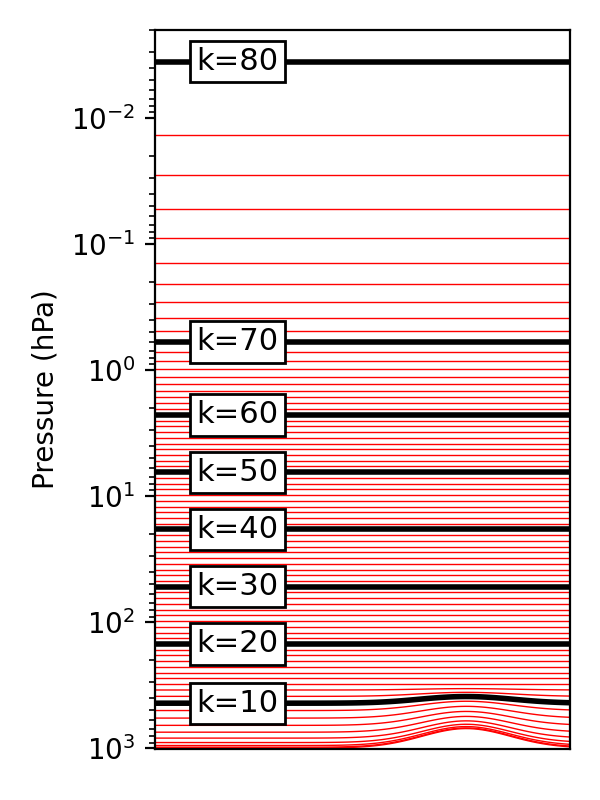
\includegraphics{levels.png}
\caption{鉛直80層とする場合のデフォルトの層配置}
\end{figure}

Each predictor is entirely defined on a grid of
\((\lambda_i, \varphi_j, \sigma_k)\) or \((\lambda_i, \varphi_j, z_l)\).
(The underground level, \(z_l\), is described in the section on physical
processes.)

In the time direction, the predictive equations are discretized at
evenly spaced \(\Delta t\) and time integration is performed. However,
if the stability of the time integration may be impaired, the
\(\Delta t\) may change.

\hypertarget{physical-constants}{%
\subsubsection{Physical Constants}\label{physical-constants}}

The basic physical constants are shown below
\texttt{MODULE:{[}APCON{]}}.

\setlength\LTleft{0pt}\setlength\LTright{0pt}\begin{longtable}[]{@{}
  >{\raggedright\arraybackslash}p{(\columnwidth - 6\tabcolsep) * \real{0.25}}
  >{\raggedright\arraybackslash}p{(\columnwidth - 6\tabcolsep) * \real{0.25}}
  >{\raggedright\arraybackslash}p{(\columnwidth - 6\tabcolsep) * \real{0.25}}
  >{\raggedright\arraybackslash}p{(\columnwidth - 6\tabcolsep) * \real{0.25}}@{}}
\toprule\relax
Header0 & Header1 & Header2 & Header3 \\
\midrule\relax
\endhead
earth radius & \(a\) & m & 6.37 \(\times 10^6\) \\
acceleration of gravity & \(g\) & ms\(^-2\) & 9.8 \\
atmospheric pressure specific heat & \(C_p\) & J kg\(^{-1}\) K\(^{-1}\)
& 1004.6 \\
Atmospheric gas constant & \(R\) & J kg\(^{-1}\) K\(^{-1}\) & 287.04 \\
Latent heat of water evaporation & \(L\) & J kg\(^{-1}\) & 2.5
\(\times 10^6\) \\
Water vapor constant pressure specific heat & \(C_v\) & J kg\(^{-1}\)
K\(^{-1}\) & 1810. \\
Gas constant of water & \(R_v\) & J kg\(^{-1}\) K\(^{-1}\) & 461. \\
Density of liquid water & \(d_{H_2O}\) & J kg\(^{-1}\) K\(^{-1}\) &
1000. \\
0 Saturated vapor at 0 \(^{\circ}\) & \(e^*\)(273K) & Pa. & 611 \\
Stefan Bolzman Constant & \(\sigma_{SB}\) & W m\(^{-2}\) K\(^{-4}\) &
5.67 \(\times 10^{-8}\) \\
Kárman Constant & \(k\) & & 0.4 \\
Latent heat of ice melting & \(L_M\) & J kg\(^{-1}\) & 3.4
\(\times 10^5\) \\
Water Freezing Point & \(T_M\) & K & 273.15 \\
Constant pressure specific heat of water & \(C_w\) & J kg\(^{-1}\) &
4,200. \\
The freezing point of seawater & \(T_I\) & K & 271.35 \\
Specific heat ratio of ice at constant pressure &
\(C_I = C_w - L_M/T_M\) & & 2397. \\
water vapor molecular weight ratio & \(\epsilon = R/R_v\) & & 0.622 \\
coefficient of provisional temperature &
\(\epsilon_v = \epsilon^{-1} - 1\) & & 0.606 \\
Ratio of specific heat to gas constant & \(\kappa = R/C_p\) & & 0.286 \\
\bottomrule
\end{longtable}
